% !TEX TS-program = pdflatex
% !TEX encoding = UTF-8 Unicode

% This is a simple template for a LaTeX document using the "article" class.
% See "book", "report", "letter" for other types of document.

\documentclass[11pt]{article} % use larger type; default would be 10pt

\usepackage[utf8]{inputenc} % set input encoding (not needed with XeLaTeX)

%%% Examples of Article customizations
% These packages are optional, depending whether you want the features they provide.
% See the LaTeX Companion or other references for full information.

%%% PAGE DIMENSIONS
\usepackage{geometry} % to change the page dimensions
\geometry{a4paper} % or letterpaper (US) or a5paper or....
% \geometry{margin=2in} % for example, change the margins to 2 inches all round
% \geometry{landscape} % set up the page for landscape
%   read geometry.pdf for detailed page layout information

\usepackage{amsmath}
\usepackage{amsthm}
\usepackage{amsfonts}
\usepackage{graphicx} % support the \includegraphics command and options

% tickz includes
\usepackage{tikz}
\usepackage{pgf}
\usepackage{mathrsfs}
\usetikzlibrary{arrows}
% \usepackage[parfill]{parskip} % Activate to begin paragraphs with an empty line rather than an indent

%%% PACKAGES
\usepackage{bbm}
\usepackage{booktabs} % for much better looking tables
\usepackage{array} % for better arrays (eg matrices) in maths
\usepackage{paralist} % very flexible & customisable lists (eg. enumerate/itemize, etc.)
\usepackage{verbatim} % adds environment for commenting out blocks of text & for better verbatim
\usepackage{subfig} % make it possible to include more than one captioned figure/table in a single float
% These packages are all incorporated in the memoir class to one degree or another...
\usepackage{amsthm}

%%% HEADERS & FOOTERS
\usepackage{fancyhdr} % This should be set AFTER setting up the page geometry
\pagestyle{fancy} % options: empty , plain , fancy
\renewcommand{\headrulewidth}{0pt} % customise the layout...
\lhead{}\chead{}\rhead{}
\lfoot{}\cfoot{\thepage}\rfoot{}

%%% SECTION TITLE APPEARANCE
\usepackage{sectsty}
\allsectionsfont{\sffamily\mdseries\upshape} % (See the fntguide.pdf for font help)
% (This matches ConTeXt defaults)

%%% ToC (table of contents) APPEARANCE
\usepackage[nottoc,notlof,notlot]{tocbibind} % Put the bibliography in the ToC
\usepackage[titles,subfigure]{tocloft} % Alter the style of the Table of Contents
\renewcommand{\cftsecfont}{\rmfamily\mdseries\upshape}
\renewcommand{\cftsecpagefont}{\rmfamily\mdseries\upshape} % No bold!
\usetikzlibrary{arrows.meta}
\usetikzlibrary{svg.path}
%%% END Article customizations

%%% The "real" document content comes below...

\title{Some Presentations of Planar Algebras with Applications to Invariant Theory}
\author{Ryan Vitale}
%\date{} % Activate to display a given date or no date (if empty),
         % otherwise the current date is printed 



%%% Macros

\newcommand{\repz}{Rep$_{K,1}(\mathbb{Z})$}
\newcommand{\h}[2]{\{#1..#2\}}


%\newcommand{\dotmap}{
%\begin{tikzpicture}
%\draw [line width=1.1pt] (0,0) -- (0,1.5ex);
%\draw [fill=black] (0,1.5ex) circle (0.7pt); 
%\end{tikzpicture}
%}

%\newcommand{\lcap}{
%\begin{tikzpicture}
%\draw [line width=1.1pt] (0,0) -- (0,1.75ex);
%\draw [line width=1.1pt] (0,1.75ex) -- (0.5ex,1.75ex);
%\end{tikzpicture}
%}

\newcommand{\lcap}{\boldmath$\langle$\unboldmath}
\newcommand{\rcap}{\boldmath$\rangle$\unboldmath}
\newcommand{\dotmap}{$\bullet$}

%\newcommand{\rcap}{
%\begin{tikzpicture}
%\draw [line width=1.1pt] (0.5ex,0) -- (0.5ex,1.75ex);
%\draw [line width=1.1pt] (0.5ex,1.75ex) -- (0,1.75ex);
%\end{tikzpicture}
%}

\usetikzlibrary{decorations.markings}
\usetikzlibrary{arrows.meta}

\begin{document}

\newtheorem{mydef}{Definition}
\newtheorem{prop}{Proposition}
\newtheorem{lemma}{Lemma}

\maketitle

\section{Introduction}

Fix a group $G$, a field $k$, and some object $V\in \text{Rep}_k(G)$, the category of $k$-linear representations of $G$. We study $\text{Alg}_{(G,V,k)}$, the full subcategory of $\text{Rep}_k(G)$ whose objects are finite tensor products of $V$ and $V^{\ast}$. We denote by $M_{G,V,k}$ the morphisms of $\text{Alg}_{(G,V,k)}$, and by $P_{G,V,k}$ the planar algebra structure on $M_{G,V,k}$. Our goal will be to give a diagrammatic presentation of $P_{G,V,k}$. In all examples considered it will be true that $V \simeq V^{\ast}$, so we can restrict to studying the spaces $\text{Hom}(V^{\otimes n},V^{\otimes m})$. Further, since $\text{Hom}(A, B \otimes C) \simeq \text{Hom}(A\otimes B^{\ast},C)$ for $A,B,C$ finite dimensional representations of a group, we can restrict to studying the spaces $B_n := \text{Hom}(V^{\otimes n}, \mathbbm{1})$.

Diagrammatically, we have oriented strands connecting function blocks. We will assign an upwards oriented strand to the identity map on $V$ and a downward oriented strand to the identity map on $V^{\ast}$, keeping track of the type of data flowing along a strand and consequently the type of inputs and outputs to function blocks. We have evaluation and coevaluation maps $V^{\ast} \otimes V \xrightarrow{\epsilon} k$, $k \xrightarrow{\eta} V \otimes V^{\ast}$ drawn by arcs connecting appropriately oriented strands. We fix an isomorphism $\varphi:V \xrightarrow{\sim} V^{\ast}$ and draw this between the upward and downward oriented strand.

\begin{tikzpicture}[scale=0.9]
\clip (-2,2.9) rectangle (16,5.8);
\begin{scope}[decoration={
    markings,
    mark=at position 0.5 with {\arrow[scale=1.25]{latex}}}
    ]
\draw [-,postaction={decorate}] (0,3) to (0,5.5);
\draw (0.5,4.25) node[scale=1.25] {$\leadsto$};

\draw [-,postaction={decorate}] (3,5.5) to (3,3);
\draw (3.5,4.25) node[scale=1.25] {$\leadsto$};

\draw (1.2,4.25) node {$\text{Id}_V$};
\draw (4.2,4.25) node {$\text{Id}_{V^{\ast}}$};

\draw [-,postaction={decorate}] (7.25,3) to  [controls=+(90:1) and +(90:1)] (5.75,3);

\draw [-,postaction={decorate}] (7.25,5.5) to  [controls=+(-90:1) and +(-90:1)] (5.75,5.5);

\draw (7.75,3.25) node[scale=1.25] {$\leadsto \eta$};
\draw (7.75,5) node[scale=1.25] {$\leadsto \epsilon$};

\draw (9.5,4) rectangle (10,4.5);
\draw (9.75,4.25) node {$\varphi$};

\draw [-,postaction={decorate}] (9.75,3) to (9.75,4);
\draw [-,postaction={decorate}] (9.75,5.5) to (9.75,4.5);

\draw (10.6,4.2) node[scale=1.25] {$\leadsto \varphi$};

\end{scope}
\end{tikzpicture}


Using $\varphi$ along with evaluation we can turn outgoing strands into incoming ones, illustrating the isomorphism $\text{Hom}(V^{\otimes n},V^{\otimes m}) \xrightarrow{\sim} \text{Hom}(V^{\otimes (n+m)}, \mathbbm{1})$, and allowing us to focus on pictures where all strands are `attached to the ground'.

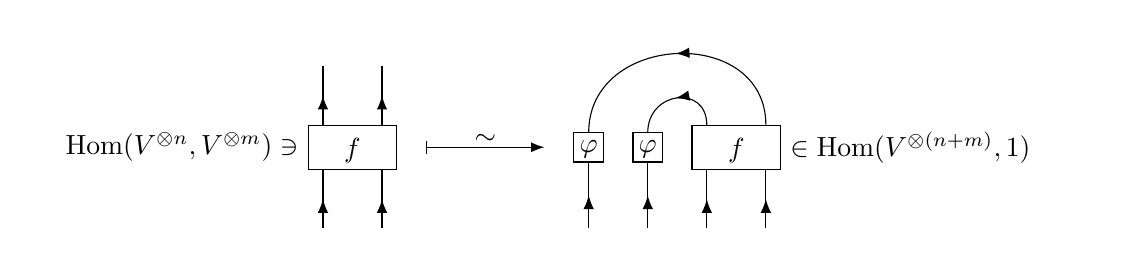
\begin{tikzpicture}[x=0.75cm,y=0.75cm]
\clip (-2.5,-.1) rectangle (16,3.4);
\begin{scope}[decoration={
    markings,
    mark=at position 0.5 with {\arrow[scale=1.25]{latex}}}
    ]

\draw (2.25,1) rectangle (3.75,1.75);
\draw (3, 1.325) node {$f$};

\draw (2.25,1.375) node[anchor=east] {$\text{Hom}(V^{\otimes n}, V^{\otimes m}) \ni $};

\draw [|->,>=Latex] (4.25,1.375) to (6.25,1.375);

\draw (5.25,1.5) node {$\sim$};


\draw (8.75,1) rectangle (10.25,1.75);

\draw (9.5, 1.325) node {$f$};

\draw (6.75,1.125) rectangle (7.25,1.625);
\draw (7.75,1.125) rectangle (8.25,1.625);

\draw (7,1.35) node {$\varphi$};
\draw (8,1.35) node {$\varphi$};

\draw [-,postaction={decorate}] (9,1.75) to [controls=+(90:0.7) and +(90:0.7)] (8,1.625);
\draw [-,postaction={decorate}] (10,1.75) to [controls=+(90:1.7) and +(90:1.7)] (7,1.625);

\foreach \x in {2.5,3.5,9,10}
	\draw [-,postaction={decorate}] (\x,0) to (\x,1);
	
\foreach \x in {7,8}
	\draw [-,postaction={decorate}] (\x,0) to (\x,1.125);

\foreach \x in {2.5,3.5}
	\draw [-,postaction={decorate}] (\x,1.75) to (\x,2.75);

\draw (10.25,1.375) node[anchor=west] {$ \in \text{Hom}(V^{\otimes (n+m)},\mathbbm{1})$};

% cap rhs with varphi isos

\end{scope}
\end{tikzpicture}

 Our goal is to determine a minimal generating set of pictures and relations so that the resulting diagrammatic planar algebra, call it $\text{Diag}_{(G,V,k)}$, will be isomorphic to $P_{G,V,k}$. In each example we use the following procedure:
 \begin{enumerate}
 \item Define generating pictures and relations for $\text{Diag}_{(G,V,k)}$, and give a map of planar algebras $\text{Diag}_{(G,V,k)} \xrightarrow{T} P_{G,V,k}$.
 \item For each $n$ find a subset $D_n \subset \text{Diag}_{(G,V,k)}$ such that $T(D_n)$ is a basis for $B_n$. Exhibiting such $D_n$ shows that $T$ is surjective, since as argued above $M_{G,V,k}$ is determined by the spaces $B_n$.
 \item Show that an arbitrary picture in $\text{Diag}_{(G,V,k)}$ can be rewritten linearly in terms of elements of the $D_n$ using the presented relations. This shows that $T$ is injective, so that $\text{Diag}_{(G,V,k)} \simeq P_{G,V,k}$ as planar algebras. 
 
 \end{enumerate}

If we fix coordinates on $V$, when describing the spaces $B_n$ we are also describing a subring of vector invariants for $G$, i.e. each $f$ in $B_n$ is also in $(V^{\oplus n})^G=\{f \in k[x_1,\ldots,x_n] : \forall g \in G, f(\bar{x}) = f(g \cdot \bar{x})\}$. This follows from observing that the defining property for an element of $(V^{\oplus n})^G$ is the same as the defining property for a map of $G$ representations from $V^{\otimes n}$ to the trivial representation. Giving a presentation of $\text{Alg}_{(G,V,k)}$ is then related to giving a first and second fundamental theorem of invariant theory for $(V^{\oplus n})^G$, and in each example we discuss this relationship.


\section{A 2-dimensional $\mathbb{Z}$-representation over $\mathbb{C}$}

Let $V_n=(\mathbb{C}^n,\phi_n)$ where $\phi_n: \mathbb{Z} \rightarrow GL(\mathbb{C}^n)$ is defined by $\phi_n(1)=J_n$, and $J_n$ is the Jordan block of dimension $n$ with eigenvalue $1$. In this section we set $V=V_2$ and study $\text{Alg}_{\mathbb{Z},V, \mathbb{C}}$. Taking the standard basis of $\mathbb{C}^2$, $v_0 = (1,0)$ and  $v_1 = (0,1)$, we use the isomorphism $\varphi:V \xrightarrow{\sim} V^{\ast}$ defined by $\varphi(v_0)=v_1^{\ast}$, $\varphi(v_1)=-v_0^{\ast}$. We want to describe the spaces $B_n = \text{Hom}(V^{\otimes n},\mathbbm{1} \simeq V_1)$.

\subsection {Presentation of $\text{Diag}_{(\mathbb{Z},V,\mathbb{C})}$ and map into $\text{Alg}_{(\mathbb{Z},V,\mathbb{C})}$}

\begin{mydef}
We present $\text{Diag}_{(\mathbb{Z},V,\mathbb{C})}$ by the generators and relations below:
\end{mydef}

\begin{tikzpicture}
\begin{scope}[decoration={
    markings,
    mark=at position 0.5 with {\arrow[scale=1.25]{latex}}}
    ]
\clip (-1,-1.25) rectangle (16,4);

\draw [postaction={decorate}] (0,0) circle (17pt);
\draw (1.2,0) node[scale=1.4] {$=$};
\draw (1.2,.05) node[anchor=south,scale=0.8] {$R_3$};
\draw (1.5,.05) node[anchor=west,scale=1.4] {$2$};
\draw [dotted] (-0.9,-1) rectangle (2.25,1);


\draw [-,postaction=decorate] (9.25,-0.75) to (9.25,0.75);
\draw [-,postaction=decorate] (9.75,-0.75) to (9.75,0.75);
\draw (10.25,0) node[scale=1.2] {$+$};

%\draw (0,3) node[anchor=west] {\textbf{Generators:}};
\draw [-,postaction={decorate}] (0,1.5) to (0,2.75);
\draw [fill=black] (0,2.75) circle (1.5pt);

\draw [-,postaction={decorate}] (8,3.25) to (8,1.5);
\draw (7,2.25) node[scale=1.4] {$=$};
\draw (7,2.3) node[anchor=south,scale=0.8] {$R_1$};

\draw [dotted] (5.5,1.25) rectangle (8.5,3.5);
\end{scope}

\draw (-0.1,2.25) node[anchor=east] {$G_1:$};

\begin{scope}[decoration={
	markings,
	mark=at position 0.5 with {\arrow[scale=1.25,thick]{[}},
	mark=at position 0.25 with {\arrow[scale=1.25]{latex}},
	mark=at position 0.8 with {\arrow[scale=1.25,>=latex]{<}}}
	]

\draw [-,postaction={decorate}] (2,3.25) to (2,1.5);
\draw [-,postaction={decorate}] (3.5,-0.75) to (3.5,0.75);
\draw [-,postaction={decorate}] (5.5,0.75) to (5.5,-0.75);

\draw (4.5,0) node[scale=1.4] {$=$};
\draw (4.5,0.05) node[scale=0.8,anchor=south] {$R_4$};
\draw (5,0) node[scale=1.2] {$-$};
\draw [dotted] (3,-1) rectangle (6,1);

\draw [dotted] (6.5,-1) rectangle (12.25,1);
\end{scope}

\draw (1.9,2.25) node[anchor=east] {$G_2:$};


\begin{scope}[decoration={
	markings,
	mark=at position 0.5 with {\arrow[scale=1.25,thick]{]}},
	mark=at position 0.8 with {\arrow[scale=1.25]{latex}},
	mark=at position 0.25 with {\arrow[scale=1.25,>=latex]{<}}}
	]
\draw [-,postaction={decorate}] (4,3.25) to (4,1.5);

\draw [-,postaction={decorate}] (10,3.25) to (10,1.5);
\draw [fill=black] (10,3.25) circle (1.5pt);
\draw [fill=black] (10,1.5) circle (1.5pt);
\draw (11,2.25) node[scale=1.4] {$=$};
\draw (11,2.3) node[anchor=south,scale=0.8] {$R_2$};
\draw (11.5,2.3) node[scale=1.3,anchor=west] {$0$};
\draw [dotted] (9.5,1.25) rectangle (12.25,3.5);

\end{scope}

\begin{scope}[decoration={markings,
	mark=at position 0.35 with {\arrow[scale=1.25,thick]{]}},
	mark=at position 0.55 with {\arrow[scale=1.25,>=latex]{>}},
	mark=at position 0.2 with {\arrow[scale=1.25,>=latex]{<}}}
	]
\draw [-,postaction=decorate] (12,.75) to [controls= +(-90:0.75) and +(-90:0.75)] (10.75,0.7);
\end{scope}
\begin{scope}[decoration={markings,
	mark=at position 0.35 with {\arrow[scale=1.25,thick]{]}},
	mark=at position 0.55 with {\arrow[scale=1.25,>=latex]{<}},
	mark=at position 0.2 with {\arrow[scale=1.25,>=latex]{>}}}
	]
\draw [-,postaction=decorate] (10.75,-0.75) to [controls= +(90:0.75) and +(90:0.75)] (12,-0.75);
\end{scope}

\begin{scope}[decoration={
	markings,
	mark=at position 0.3 with {\arrow[scale=1.25]{latex}},
	mark=at position 0.8 with {\arrow[scale=1.25]{latex}}}
	]

\draw [-,postaction={decorate}] (6.75,-0.75) to (8,0.75);
\draw [-,postaction={decorate}] (8,-0.75) to (6.75,0.75);	

\end{scope}


%\draw [-,postaction={decoration={markings,mark=at position 0.5 with {\arrow{latex}},mark=at position 0.6 with {\arrow{Latex}}},decorate}] (1,1) to (2,2);

\draw [-,postaction={decoration={markings,mark=at position 0.35 with {\arrow[scale=1.25,thick]{[}},mark=at position 0.65 with {\arrow[scale=1.25,thick]{]}},mark=at position 0.2 with {\arrow[scale=1.25,>=latex]{<}},mark=at position 0.8 with {\arrow[scale=1.25,>=latex]{<}},mark=at position 0.53 with {\arrow[scale=1.25,>=latex]{>}}},decorate}] (6,1.5) to (6,3.25);




\draw (3.9,2.25) node[anchor=east] {$G_3:$};



\draw (8.5,0) node[scale=1.4] {$=$};
\draw (8.5,0.05) node[scale=0.8,anchor=south] {$R_5$};





\end{tikzpicture}


\begin{prop}
There is a map of planar algebras $T:\text{Diag}_{(\mathbb{Z},V,\mathbb{C})} \rightarrow \text{Alg}_{(\mathbb{Z},V,\mathbb{C})}$ determined by the values $T(G_1)=v_1^{\ast},T(G_2)=\varphi$ and $T(G_3)=\varphi^{-1}$. 
\end{prop}

\begin{proof}
We need to show each of $R_1$ through $R_5$ hold in the image of $T$ so that this map is well defined.

\begin{enumerate}[$R_1$:]
\item $\varphi \cdot \varphi^{-1} = \text{Id}_{V^{\ast}}$
\item $1 \mapsto v_1^{\ast} \mapsto v_0 \mapsto 0$
\item $\epsilon \cdot \tau \cdot \eta(1) = \epsilon \cdot \tau (v_1 \otimes v_1^{\ast} + v_0 \otimes v_0^{\ast})=\epsilon(v_1^{\ast} \otimes v_1 + v_0^{\ast} \otimes v_0) = 2$
\item This follows from taking the dual (rotation) of $G_2$ and a coordinate computation:

\begin{tikzpicture}
\clip (-3,0) rectangle (15,2.5);

\begin{scope}[decoration={
	markings,
	mark=at position 0.5 with {\arrow[scale=1.25,thick]{]}},
	mark=at position 0.8 with {\arrow[scale=1.25,>=latex]{<}},
	mark=at position 0.25 with {\arrow[scale=1.25,>=latex]{>}}}
	]

\draw [-,postaction={decorate}] (1,0) to (1,2);

\draw (1.3,2) node {$*$};

\draw (2,1) node {$=$};

\draw [-,postaction={decorate}] (3.5,0.25) to (3.5,1.75);

\draw (3,0.25) to [controls= +(270:0.3) and +(-90:0.3)] (3.5,0.25);
\draw (3.5,1.75) to [controls= +(90:0.3) and +(90:0.3)] (4,1.75);

\draw (3,2) to (3,0.25);
\draw (4,1.75) to (4,0);

\draw (5,1) node {$=$};

\draw [-,postaction={decorate}] (6,2) to (6,0);

\end{scope}

\end{tikzpicture}

\begin{align*}
(&\text{Id}_{V^{\ast}}\otimes \epsilon)(\text{Id}_{V^\ast} \otimes \varphi \otimes \text{Id}_V)(\tau \cdot \eta \otimes \text{Id}_V)(v_0) & &= \\
(&\text{Id}_{V^{\ast}}\otimes \epsilon)(\text{Id}_{V^\ast} \otimes \varphi \otimes \text{Id}_V)(v_0^{\ast} \otimes v_0 \otimes v_0 + v_1^{\ast} \otimes v_1 \otimes v_0) & &= \\
(&\text{Id}_{V^{\ast}}\otimes \epsilon)(v_0^{\ast} \otimes v_1^{\ast} \otimes v_0 - v_1^{\ast} \otimes v_0^{\ast} \otimes v_0) & &= -v_1^{\ast} \\
\end{align*}
\begin{align*}
(&\text{Id}_{V^{\ast}}\otimes \epsilon)(\text{Id}_{V^\ast} \otimes \varphi \otimes \text{Id}_V)(\tau \cdot \eta \otimes \text{Id}_V)(v_1) & &= \\
(&\text{Id}_{V^{\ast}}\otimes \epsilon)(\text{Id}_{V^\ast} \otimes \varphi \otimes \text{Id}_V)(v_0^{\ast} \otimes v_0 \otimes v_1 + v_1^{\ast} \otimes v_1 \otimes v_1) & &= \\
(&\text{Id}_{V^{\ast}}\otimes \epsilon)(v_0^{\ast} \otimes v_1^{\ast} \otimes v_1 - v_1^{\ast} \otimes v_0^{\ast} \otimes v_1) & &= v_0^{\ast}\\
\end{align*}

\item The second term on the RHS takes the values $v_0 \otimes v_0 \mapsto 0, v_1 \otimes v_1 \mapsto 0, v_0 \otimes v_1 \mapsto v_1 \otimes v_0 - v_0 \otimes v_1, v_1 \otimes v_0 \mapsto v_0 \otimes v_1 - v_1 \otimes v_0$, and adding the identity map gives us the LHS.
\end{enumerate}

\end{proof}

\subsection{Exhibiting bases $D_n$ for each $B_n$}

The indecomposable representations that appear in $\otimes$-powers of $V$ are exhausted by the sequence $V_n$. When $i \geq 2$ we have the rule

\begin{equation} \label{eq1}
V \otimes V_i \simeq V_{i+1} \oplus V_{i-1}
\end{equation}

so that the fusion graph $\Gamma$ for $V$ is

\begin{tikzpicture}
\clip(-0.5,-1.85) rectangle (14,-.25);
\foreach \x in {1,...,7}
	\draw (2*\x-2,-1.1) node[anchor=north] {$V_{\x}$};
\foreach \x in {1,...,6}
	{\draw [->, >=latex] (2*\x-2,-1) to (2*\x-0.1,-1);
	\draw [<-, >=latex] (2*\x-1.9,-1) to (2*\x,-1);}
\draw (12,-1) to (13,-1);

\foreach \x in {0,...,6}
	\draw [fill=black] (2*\x,-1) circle (2pt);
\foreach \x in {1,...,3}
	\draw [fill=black] (13+.25*\x,-1) circle (0.5pt);

\draw [->,>=latex] (12.5,-1) to (12.1,-1);

\end{tikzpicture}

\begin{mydef}
Let $P_n$ be the set of paths of length $n$ on $\Gamma$ based at $V_1$. Label edges directed from $V_i$ to $V_{i+1}$ with $R$, and edges directed from $V_{i}$ to $V_{i-1}$ by $L$. Then we can describe $P_n$ as the set of words $w$ of length $n$ in the alphabet $\{R,L\}$ where no initial segment of $w$ has more $L$s than $R$s.
\end{mydef}

\begin{prop}
$\#(P_n)=dim(B_n)$
\end{prop}

\begin{proof}
  We have $\dim(B_n)=\text{dimHom}(V^{\otimes n},\mathbbm{1})=\text{dimHom} \big( \sum{\alpha_i V_i,\mathbbm{1} \big) }=\sum{\alpha_i \text{dimHom}(V_i,\mathbbm{1})}$. Since dimHom$(V_j, \mathbbm{1}) = 1$ for any indecomposable $V_j$, we get dim$(B_n)=\sum{\alpha_i}$, which is the number of summands of $V^{\otimes n}$. We can see summands of $V^{\otimes n}$ are in bijection with $P_n$ by induction on $n$. Assume we have a direct sum decomposition of $V^{\otimes n}$ and a bijection between summands of $V^{\otimes n}$ and $P_n$. By definition of $\Gamma$ the summands of $V^{\otimes (n+1)}$ will be the indecomposables that are adjacent to the summands of $V^{\otimes n}$, so append the adjacency edge to the path from the bijection at level $n$.
\end{proof}

We will then construct a set of maps in bijection with $P_n$, and show these maps are independent, so that this set forms a basis for $B_n$. We first construct a map from the set of paths to the diagrammatic category.
\begin{mydef}
We define a map $\delta_n :P_n \rightarrow \text{Diag}_{(\mathbb{Z},V,\mathbb{C})}$. Identify concatenation in a path word $w$ with composition of diagrams, and identify each letter of the alphabet with a portion of a picture as below, where $\emptyset$ signifies the end of the word.

\begin{tikzpicture}[x=.6cm,y=.6cm]
\clip(-3,-0.5) rectangle (20,5);
\begin{scope}[decoration={
    markings,
    mark=at position 0.5 with {\arrow[scale=1.25]{latex}}}
    ]

\draw [dotted] (1,0) rectangle (5,4);
\draw [-,postaction={decorate}] (1,2) to (5,2);
\draw [-,postaction={decorate}] (1,3) to (5,3);
\draw [fill=black] (3,2.25) circle (0.5pt);
\draw [fill=black] (3,2.50) circle (0.5pt);
\draw [fill=black] (3,2.75) circle (0.5pt);
\draw (3,4) node[anchor=south] {$R$};
\draw [-,postaction={decorate}] (3,0) to [controls = +(270:-1) and +(0:-1)] (5,1.5);


\draw [dotted] (6,0) rectangle (10,4);
\draw [-,postaction={decorate}] (6,2) to (10,2);
\draw [-,postaction={decorate}] (6,3) to (10,3);
\draw [fill=black] (8,2.25) circle (0.5pt);
\draw [fill=black] (8,2.5) circle (0.5pt);
\draw [fill=black] (8,2.75) circle (0.5pt);
\end{scope}
\begin{scope}[decoration={
    markings,
    mark=at position 0.5 with {\arrow[scale=1.25,thick]{]}},
    mark=at position 0.25 with {\arrow[scale=1.25]{latex}},
    mark=at position 0.75 with {\arrow[scale=1.25,>=latex]{<}}}
    ]

\draw [-,postaction={decorate}] (8,0) to [controls = +(270:-1) and +(0:1)] (6,1.5);
\end{scope}
\begin{scope}[decoration={
	markings,
	mark=at position 0.45 with {\arrow[scale=1.25]{latex}}}
	]
\draw (8,4) node[anchor=south] {$L$};

\draw [dotted] (11,0) rectangle (15,4);
\draw (13,4) node[anchor=south] {$\emptyset$};


\draw [-,postaction={decorate}] (11,3) to [bend right] (12,3.5);
\draw [-,postaction={decorate}] (11,2) to [bend right] (12.25,2.5);
\draw [fill=black] (12,3.5) circle (1.5pt);
\draw [fill=black] (12.25,2.5) circle (1.5pt);

\draw [fill=black] (11.5,2.25) circle (0.5pt);
\draw [fill=black] (11.5,2.5) circle (0.5pt);
\draw [fill=black] (11.5,2.75) circle (0.5pt);

\end{scope}
\end{tikzpicture}

The number of horiztonal strands in each picture varies, and is equal to the excess of $R$s to $L$s in the segment prior to the current letter of $w$. To define $\delta_n(w)$ replace each letter of $w$ with its identified picture, and then glue each portion end to end, including the picture for $\emptyset$ at the end (glue dots onto any remaining strands at the end).
\end{mydef}

For example, take $w=RRRLLRL$:

\begin{tikzpicture}[x=1.1cm]
\clip (-1.51,-0.5) rectangle (16,1.7);

\draw [dotted] (0,0) rectangle (8,1.5);
\foreach \x in {1,...,7}
	\draw [dotted] (\x,0) to (\x,1.5);
\draw (-1.5,.75) node[anchor=west] {$\delta_7(w)=$};
\draw (8,.75) node[anchor=west] {$=$};
\foreach \x in {1,2,3,6}
	\draw (-0.5 + \x,0) node[anchor=north] {$R$};
\foreach \x in {4,5,7}
	\draw (-0.5 + \x,0) node[anchor=north] {$L$};

\draw (7.5,0) node[anchor=north] {$\emptyset$};

\begin{scope}[decoration={
    markings,
    mark=at position 0.5 with {\arrow{latex}}}
    ]

\draw [-,postaction={decorate}] (0.5,0) to [controls= +(90:0.5) and +(180:0.3)] (1,0.9);
\draw [-,postaction={decorate}] (1.5,0) to [controls= +(90:0.35) and +(180:0.3)] (2,0.7);
\draw [-,postaction={decorate}] (2.5,0) to [controls= +(90:0.2) and +(180:0.3)] (3,0.5);
\foreach \x in {1,...,6}
	\draw [-,postaction={decorate}] (\x,0.9) to (\x+1,0.9);

\draw [-,postaction={decorate}] (2,0.7) to (3,0.7);
\draw [-,postaction={decorate}] (3,0.7) to (4,0.7);

\draw [-,postaction={decorate}] (5.5,0) to [controls = +(90:0.2) and +(180:0.3)] (6,0.5);

\draw [-,postaction={decorate}] (7,0.9) to [bend right] (7.4,1.2);

\draw [fill=black] (7.4,1.2) circle (1.25pt);

\draw [-,postaction={decorate}] (8.85,0) to (8.85,0.6);
\draw [fill=black] (8.85,0.6) circle (1.25pt);

\end{scope}
\begin{scope}[decoration={
	markings,
	mark=at position 0.5 with {\arrow[thick]{]}},
	mark=at position 0.3 with {\arrow[>=latex]{>}},
	mark=at position 0.8 with {\arrow[>=latex]{<}}}
	]

\draw [-,postaction={decorate}] (6.5,0) to [controls= +(90:0.3) and +(0:0.3)] (6,0.5);
\draw [-,postaction={decorate}] (4.5,0) to [controls= +(90:0.4) and +(0:0.4)] (4,0.7);
\draw [-,postaction={decorate}] (3.5,0) to [controls= +(90:0.3) and +(0:0.3)] (3,0.5);

\end{scope}

\begin{scope}[decoration={
	markings,
	mark=at position 0.75 with {\arrow[thick]{]}},
	mark=at position 0.65 with {\arrow[>=latex]{>}},
	mark=at position 0.9 with {\arrow[>=latex]{<}}}
	]

\draw [-,postaction={decorate}] (10.25,0) to [controls = +(90:0.5) and +(90:0.5)] (9.5,0);
\draw [-,postaction={decorate}] (10.5,0) to [controls = +(90:0.9) and +(90:0.9)] (9.25,0);
\draw [-,postaction={decorate}] (11.5,0) to [controls = +(90:0.5) and +(90:0.5)] (10.75,0);

\end{scope}
\end{tikzpicture}
 

The images of $\delta_n$ form our sequence $D_n$. Composing $\delta_n$ with $T$ we get $T_n:P_n \rightarrow B_n$. We want to show the values of $T_n$ are linearly independent. The following fact from linear algebra will be useful.

\begin{lemma} Let $(S,<)$ be a finite ordered set, and $V$ a vector space. If there are maps $f:S \rightarrow V$ and $g:S \rightarrow V^*$ such that for all $x,y \in S$:
\begin{enumerate}
\item $g(x)(f(x)) \neq 0$
\item $x<y \implies g(x)(f(y))=0$
\end{enumerate}
Then both the values of $f$ and the values of $g$ are linearly independent.
\end{lemma}
\begin{proof}
For simplicity replace $S$ with the ordered set $(1,2,\dots,n)$. Consider the $n \times n$ matrix $A$ defined by $A_{i,j}=g(i)(f(j))$. Condition $(1)$ implies entries on the main diagonal of $A$ are non-zero. Condition $(2)$ implies $A$ is upper triangular, so together $(1)$ and $(2)$ imply $A$ is invertible. Any linear dependence among the rows of $A$ implies a linear dependence among the values of $g$, and a dependence among columns of $A$ implies a dependence among the values of $f$, so we have our result.
\end{proof}
\begin{prop}
The values of $T_n$ are linearly independent. 
\end{prop}
\begin{proof}
As in Lemma 1, let $S$ be $P_n$ with lexicographic order ($R>L$), and let $g$ be $T_n$. To define $f$ assign to each $x \in P_n$ a vector $f(x) \in V^{\otimes n}$ by identifying $R$ with $v_1$, $L$ with $v_0$, and concatenation with $\otimes$ (e.g. $f(RRLRLLRL)=v_1 \otimes v_1 \otimes v_0 \otimes v_1 \otimes v_0 \otimes v_0 \otimes v_1 \otimes v_0)$. 
By construction of the pairing we have $g(x)(f(x))=1$, so condition $1$ of Lemma $1$ holds. To show condition $2$ holds, note that if $x<y$ then
\begin{align*} 
f(y) &= v_1^{\otimes i} \otimes v_1 \otimes u, \hspace{5mm} u \in V^{\otimes (n-(i+1))} \\
f(x) &= v_1^{\otimes i} \otimes v_0 \otimes w, \hspace{5mm} w \in V^{\otimes (n-(i+1))}
\end{align*}
so that $g(x)(f(y))$ will have the form

\begin{tikzpicture}[x=1.1cm,y=0.9cm]
\clip (-3,-1) rectangle (10,2.5);
\draw (1,1) rectangle (5,2);
\draw (3,1.5) node {$h$};
\begin{scope}[decoration={
	markings,
	mark=at position 0.5 with {\arrow[>=latex]{>}}}
	]
\foreach \x in {1.25,2,4,4.75}
	\draw [-,postaction=decorate] (\x,0) to (\x,1);
\end{scope}
	
\draw (1.65,0.5) node {$\cdots$};
\draw (4.425,0.5) node {$\cdots$};

\begin{scope}[decoration={
	markings,
	mark=at position 0.8 with {\arrow[thick]{]}},
	mark=at position 0.7 with {\arrow[>=latex]{>}},
	mark=at position 0.9 with {\arrow[>=latex]{<}}}
	]

\draw [-,postaction={decorate}] (3.5,0) to [controls= +(90:0.9) and +(90:0.9)] (2.5,0);
\end{scope}

\draw (3.5,-0.25) node {$v_1$};
\draw (2.5,-0.25) node {$v_1$};

\draw (1.65,0) node[anchor=north] {$\underbrace{v_1 \cdots v_1}_{i-1}$};
\draw (4.37,0) node[anchor=north] {$\underbrace{\hspace{4mm}u \hspace{4mm}}_{n-(i+1)}$};

\end{tikzpicture}
which vanishes since looking at positions $i$ and $i+1$,  $(\epsilon)(-\varphi \otimes \text{Id}_{V})(v_1 \otimes v_1)=\epsilon(v_0^{\ast} \otimes v_1)=0$.
\end{proof}

 We then have a basis for each $B_n$ described as images of a set of diagrams $D_n \subset \text{Diag}_{(\mathbb{Z},V,\mathbb{C})}$ under the map $T$.

\subsection{Showing $D_n$ span $\text{Diag}_{(\mathbb{Z},V,\mathbb{C})}$.}

We need to give a visual description of the pictures in $D_n$, and then show if we take an arbitrary picture in $\text{Diag}_{(\mathbb{Z},V,\mathbb{C})}$ we can reduce it to the span of $D_n$. A picture is in $D_n$ if:

\begin{enumerate}
\item No part of the diagram is a map from 0 strands to 0 strands (define strand box spaces to clean this up).
\item No dot is enclosed (any dot can be stretched upwards arbitrarily far without crossing a strand)
\item There are no crossings.
\item The only decorations that occur are dots and brackets directed towards the left strand of a cap, with only one feature to a path.
\end{enumerate}

\begin{prop}
$\text{Diag}_{\mathbb{Z},V,\mathbb{C}}$ is spanned by $D_n$
\end{prop}
\begin{proof}

\end{proof}
The result of this section concludes the exhibition of a bijection $\text{Diag}_{(\mathbb{Z},V,\mathbb{C})} \rightarrow \text{Alg}_{(\mathbb{Z},V,\mathbb{C})}$.

\subsection{The Invariant space $(V^{\oplus n})^{\mathbb{Z}}$ and the Nowicki conjecture}
\section{A 2-dimensional $\mathbb{Z}_p$-representation over $\mathbb{F}_p$}

Let $V_n=({\mathbb{F}_p}^n,\phi_n)$ where $\phi_n: \mathbb{Z}_p \rightarrow GL({\mathbb{F}_p}^n)$ is defined by $\phi_n(1)=J_n$, and $J_n$ is the Jordan block of dimension $n$ with eigenvalue $1$. In this section we set $V=V_2$ and study $\text{Alg}_{\mathbb{Z},V, \mathbb{C}}$. Taking the standard basis of $\mathbb{C}^2$, $v_0 = (1,0)$ and  $v_1 = (0,1)$, we use the isomorphism $\varphi:V \xrightarrow{\sim} V^{\ast}$ defined by $\varphi(v_0)=v_1^{\ast}$, $\varphi(v_1)=-v_0^{\ast}$. We want to describe the spaces $B_n = \text{Hom}(V^{\otimes n},\mathbbm{1} \simeq V_1)$.

\subsection {Presentation of $\text{Diag}_{(\mathbb{Z},V,\mathbb{C})}$ and map into $\text{Alg}_{(\mathbb{Z},V,\mathbb{C})}$}

We will include all the generators and the relations from (Ex 1) for all $p$ in our presentation. We need one new generator and one new relation which are dependent on $p$.

\begin{mydef}
We present $D_{\mathbb{Z}_p,V,\mathbb{F}_p}$ by the same generators and relations of Definition 1, along with the new generator $G_4$ and relation $R_5$

\begin{tikzpicture}
\clip (0,-2) rectangle (15,4);
\begin{scope}[decoration={
	markings,
	mark=at position 0.3 with {\arrow[scale=1.25]{latex}}}
	]

\draw [-,postaction={decorate}] (1.5,1.5) to [controls = +(90:0.75) and +(185:1)] (3,3);
\draw [-,postaction={decorate}] (2,1.5) to [controls = +(90:0.5) and +(200:1)] (3,3);
%\draw [-,postaction={decorate}] (4,1.5) to [controls = +(90:0.5) and +(-20:1)] (3,3);
\draw [-,postaction={decorate}] (4.5,1.5) to [controls = +(90:0.75) and +(-5:1)] (3,3);

\draw (0.75,2.25) node {$G_4:$};
\draw (3.2,2) node[scale=1.25] {$\cdots$};
\draw (3,1) node {$\underbrace{\hspace{32mm}}_{2p-1}$};
\draw [fill=black] (3,3) circle (2.5pt);

\draw (1,-2) to [controls= +(90:0.75) and +(90:0.75)] (2,-2);
\draw (0.5,-2) to [controls= +(90:2) and +(90:2)] (2.5,-2);


\foreach \x in {0,1,2}
	\draw (1.5,-0.8-0.2*\x) node[scale=1.25] {$\cdot$};


\draw (4,-2) to (4,-1);
\draw (4.5,-2) to (5,-1);
\draw (5.5,-2) to (5,-1);

\draw (6.5,-2) to (7,-1);
\draw (7.5,-2) to (7,-1);
\draw (8,-2) to (8,-1);
\end{scope}
\end{tikzpicture}
\end{mydef}



































































\iffalse

\section{\repz}
Fix a field $K$ with $\textrm{char}(K) = 0$ and $K = \overline{K}$. We consider \repz, the $K$-representations of $\mathbb{Z}$ with all eigenvalues equal to $1$. Let $\varphi_n: \mathbb{Z} \rightarrow GL(K^n)$ be defined by $\varphi_n(1) = J_n$, where $J_n$ is the $n$-dimensional Jordan block for the eigenvalue $1$. If we define $L_n = (K^n,\varphi_n)$, then the sequence of representations $(L_n)_{n \in \mathbb{Z}_+}$ enumerates all isomorphism classes of indecomposable objects in \repz. In this section we give a presentation of \repz.

\subsection{Hom$(L_n,L_m)$}
We need to find the $K$-linear maps $T:K^n \rightarrow K^m$ satisfying $T \cdot J_n = J_m \cdot T$. Writing $J_i = I_i + N_i$ where $I_i$ is the $i$-dimensional identity map, we have $T \cdot (I_n + N_n) = (I_m + N_m) \cdot T$, so it is sufficient to find all $T$ such that $T \cdot N_n = N_m \cdot T$. Consider an arbitrary $T=\left(a_{i,j}\right) \in \text{Hom}(K_n,K_m)$. The matrix $N_n$ acts on $T$ on the right by shifting all columns to the right once, and sending the first column to zero. Similarly, $N_m$ acts on $T$ on the left by shifting all rows up once, and sending the last row to zero. This gives the relation $a_{i,j} = a_{i+1,j+1}$ on the coordinates of T. Since further $a_{i,1}=0$ for $i > 1$ and $a_{m,j} = 0$ for $j \geq 1$, we know all entries of $T$ below the main diagonal (the set of entries $\{a_{i,i}\}$) must be $0$, and the main diagonal will be zero when $n > m$. Every diagonal of T above the main diagonal (and including the main diagonal when $n \leq m$) will then correspond to one free parameter (Make this argument better). In general, dimHom$(L_n,L_m)=\min(n,m)$.

To give an explicit basis of Hom$(L_n,L_m)$, let $s = \min(n,m)$. We fix the standard ordered basis for both $K^n$ and $K^m$, and consider $K^s$ to be a subspace of each of $K^n$ and $K^m$ by taking the first $s$ basis vectors of $K^m$, and the last $s$ basis vectors of $K^n$. The set of maps $\{T_i\}_{0 \leq i \leq s-1}$, where $T_i$ acts by $N_s^i$ on $K^s \subseteq K^n$ and $0$ on the complement of $K^s$, forms a basis of Hom$(L_n,L_m)$. For example: 

 Hom$(L_3,L_4)$ has basis $T_0 = \begin{bmatrix}
 1 & 0 & 0 \\
 0 & 1 & 0 \\
 0 & 0 & 1 \\
 0 & 0 & 0 
\end{bmatrix}$, $T_1 = \begin{bmatrix}
 0 & 1 & 0 \\
 0 & 0 & 1 \\
0 & 0 & 0 \\
 0 & 0 & 0 
\end{bmatrix}$, $T_2 = \begin{bmatrix}
 0 & 0 & 1 \\
 0 & 0 & 0 \\
 0 & 0 & 0 \\
 0 & 0 & 0
\end{bmatrix}$

 Hom$(L_4,L_3)$ has basis $T_0 = \begin{bmatrix}
 0 & 1 & 0 & 0 \\
 0 & 0 & 1 & 0 \\
 0 & 0 & 0 & 1 \\
\end{bmatrix}$, $T_1 = \begin{bmatrix}
 0 & 0 & 1 & 0 \\
 0 & 0 & 0 & 1 \\
 0 & 0 & 0 & 0 \\
\end{bmatrix}$, $T_2 = \begin{bmatrix}
 0 & 0 & 0 & 1 \\
 0 & 0 & 0 & 0 \\
 0 & 0 & 0 & 0 \\
\end{bmatrix}$.

\subsection{Tensor generation of objects by $L_2$}
The indecomposable objects $L_n$ are subject to the relation $L_2 \otimes L_n \simeq L_{n-1} \oplus L_{n+1}$ (take $L_0 = 0$), which implies that there is exactly one copy of $L_n$ in the direct sum decomposition of $L_2^{\otimes n}$. Further, we have the map $\gamma_n: L_2^{\otimes n} \rightarrow L_2^{\otimes n}$ which restricts to the identity on $L_n$ and is $0$ elsewhere. Since the $L_n$ form a full set of indecomposables, and we have the projectors $\gamma_n$, we say that \repz \hspace{.2mm} is $\otimes$-generated by $L_2$. This lets us restrict our attention to the spaces Hom$(L_2^{\otimes n}, L_2^{\otimes m}$) when studying morphisms. Since each $L_n$ is self dual we can simplify further and only consider the spaces $B_n :=$ Hom$(L_2^{\otimes n}, L_1)$, using Hom$(A, B \otimes C) \simeq \text{Hom}(A \otimes B^{\ast},C)$.

\subsection{dim$(B_n)$}
To compute these dimensions we will use the fact from section (1.1) that dim(Hom$(L_n,L_1)) = \min(n,1) = 1$, as well as the relation  $L_2 \otimes L_n \simeq L_{n-1} \oplus L_{n+1}$. The relation allows us to construct the fusion graph for $L_2 \otimes -$ :

\begin{tikzpicture}[line cap=round,line join=round,>=triangle 45,x=1.0cm,y=1.0cm]
%\clip(-0.9320981936081559,-10.16) rectangle (13.853309402501186,6.5);
\clip(-0.5,-2.75) rectangle (14.,.5);
\draw (0,-1) node[anchor=north] {$L_1$};
\draw (2,-1) node[anchor=north] {$L_2$};
\draw (4,-1) node[anchor=north] {$L_3$};
\draw (6,-1) node[anchor=north] {$L_4$};
\draw (8,-1) node[anchor=north] {$L_5$};
\draw (10,-1) node[anchor=north] {$L_6$};
\draw (12,-1) node[anchor=north] {$L_7$};
\draw (0.,-1.)-- (13,-1.);
\begin{scriptsize}
\draw [fill=black] (2.,-1.) circle (2.5pt);
\draw [fill=black] (4.,-1.) circle (2.5pt);
\draw [fill=black] (6.,-1.) circle (2.5pt);
\draw [fill=black] (8.,-1.) circle (2.5pt);
\draw [fill=black] (0.,-1.) circle (2.5pt);
\draw [fill=black] (10.,-1.) circle (2.5pt);
\draw [fill=black] (12.,-1.) circle (2.5pt);
\draw [fill=black] (13.25,-1.) circle (0.5pt);
\draw [fill=black] (13.5,-1.) circle (0.5pt);
\draw [fill=black] (13.75,-1.) circle (0.5pt);
\end{scriptsize}
\end{tikzpicture}
The edges in the graph above are bidirectional. Since dim(Hom$(L_n,L_1)) = 1$, counting dimHom$(L_2^{\otimes n}, L_1)$ is the same as counting the walks of length $n$ on the above graph. 

\noindent \textbf{Remark:} ***don't need a reference here, just make the computation for this special case in appendix***. A valid walk on this graph of length $n$ is a meander of length $n$ with step set $S = \{1,-1\}$ and weight set $\{1,1\}$ as detailed in [1]. The corresponding generating function is then $$M(z) = \frac{2z - 1 + \sqrt{1-4z^2}}{2z(1-2z)}$$ and the coefficient of $z^n$ in $M(z)$ will be dimHom$(L_2^{\otimes n}, L_1)$. After expanding $M(z)$ and some computation we find: 
$$\text{dimHom}(L_2^{\otimes n}, L_1) = {n\choose{\left \lfloor{\frac{n}{2}}\right \rfloor}}$$

\subsection{Generators for $B_n$}

We want to give a basis for $B_n$ in terms of a minimal number of generating (by $\otimes$) maps. It will in fact be good enough to look at $B_1$ and $B_2$ to find enough maps to generate bases for all other $B_n$. To start, we take the identity map as our basis for $B_0$.

\noindent\boldmath$B_1$\unboldmath: Fix a basis $v_0 = (1,0) ,v_1 = (0,1)$ for $L_2$, so that $1 \cdot v_0 = v_0$ and $1 \cdot v_1 = v_0 + v_1$. Consider the space $B_1$. We know the dimension is $1$, so any nonzero map of representations will form a basis. We choose the map $v_0 \mapsto 0, v_1 \mapsto 1$, projection onto the second coordinate, and use the symbol \dotmap\hspace{1.25mm}to represent this map.


\noindent\boldmath$B_2$\unboldmath: From our dimension formula there should be a basis of $2$ maps. For one of them we choose the tensor product of the map from $B_1$ with itself denoting $\otimes$ by concatenation, \dotmap \dotmap. Another map is given by the negative determinant: $v_0 \otimes v_0 \mapsto 0, v_1 \otimes v_0 \mapsto 1, v_0 \otimes v_1 \mapsto -1, v_1 \otimes v_1 \mapsto 0$. We can write this more compactly as $v_i \otimes v_j \mapsto i-j$, and we use a pair of matched parenthesis \lcap\rcap\hspace{1.25mm}to denote this map. We write standard basis vectors in $L_2^{\otimes n}$ by concatenating the indices of the vectors $v_0$ and $v_1$ and using bold (e.g $v_0 \otimes v_1 \otimes v_1 \otimes v_0 \otimes v_1$ = \textbf{01101}). The values of these maps on the standard basis of $L_2^{\otimes 2}$ are:

\begin{center}
\begin{tabular}{| c | c | c |}
  \hline
   & \dotmap\dotmap & \lcap\rcap \\
  \hline			
  \textbf{00} & 0 & 0 \\
  \hline
  \textbf{01} & 0 & -1 \\
  \hline
  \textbf{10} & 0 & 1 \\
  \hline
  \textbf{11} & 1 & 0 \\
  \hline

\end{tabular}
\end{center}

We see the two maps above form a basis. 

\noindent\boldmath$B_3$\unboldmath: We are looking for a basis of dim$(B_3) = {3\choose1 }= 3$ maps. Combining the maps defined so far in $B_1$ and $B_2$ we have the 4 possible maps \dotmap\dotmap\dotmap,\dotmap\lcap\rcap,\lcap\dotmap\rcap,\lcap\rcap\dotmap, so there must be some relation between them. The values for these maps on the standard basis of $L_2^{\otimes 3}$ are:
\begin{center}
\begin{tabular}{| c | c | c | c | c |}
  \hline
   & \dotmap\dotmap\dotmap & \dotmap\lcap\rcap & \lcap\dotmap\rcap & \lcap\rcap\dotmap \\
  \hline			
  \textbf{000} & 0 & 0 & 0 & 0 \\
  \hline
  \textbf{001} & 0 & 0 & 0 & 0 \\
  \hline
  \textbf{010} & 0 & 0 & 0 & 0\\
  \hline
  \textbf{100} & 0 & 0 & 0 & 0\\
  \hline
  \textbf{110} & 0 & 1 & 1 & 0\\
  \hline
  \textbf{101} & 0 & -1 & 0 & 1\\
  \hline
  \textbf{011} & 0 & 0 & -1 & -1\\
  \hline
  \textbf{111} & 1 & 0 & 0 & 0\\
  \hline  
\end{tabular}
\end{center}

We can see that \lcap\dotmap\rcap=\dotmap\lcap\rcap+\lcap\rcap\dotmap, and the maps \dotmap\dotmap\dotmap,\dotmap\lcap\rcap,\lcap\rcap\dotmap\hspace{1.25mm}form a basis of $B_3$.

\newtheorem*{proposition}{Proposition}
\begin{proposition}
Any map in $B_n$ can be written in terms of \dotmap\hspace{1mm}and \lcap\rcap. A basis for $B_n$ is the set of all words of length $n$ in the alphabet $\{$\dotmap,\lcap,\rcap$\}$ where the \lcap\hspace{1mm}and \rcap\hspace{1mm}form balanced parentheses, and no \dotmap\hspace{1.25mm}is enclosed by a set of matching parentheses.  For example \dotmap\lcap\lcap\rcap\rcap\dotmap\lcap\rcap\hspace{1mm}is a valid word in our basis set for $B_8$, but while \lcap\lcap\rcap\dotmap\rcap\dotmap\lcap\rcap\hspace{1mm}is a valid map in $B_8$ it is not included in the basis we are constructing.
\end{proposition}

\begin{proof}
The relation \lcap\dotmap\rcap=\dotmap\lcap\rcap+\lcap\rcap\dotmap\hspace{1.25mm}tells us that any \dotmap\hspace{1.25mm}can be freed from enclosing parentheses. Denote the candidate basis of the proposition by $X_n$. We will show first that $|X_n|= \dim(B_n)$, and then that the elements of $X_n$ are linearly independent so that $X_n$ is a basis of $B_n$.


\noindent\boldmath$|X_n|= \dim(B_n)$\unboldmath: As in section (1.3), $B_n$ is enumerated by the set of meanders of length $n$ in steps of $1$ or $-1$, which we will denote $M_n$. Any element of $M_n$ can be identified with an element of $\{\pm{1}\}^n$. Define $\varphi: X_n \rightarrow M_n$ by \dotmap $\mapsto$$1$, \lcap $\mapsto$$1$, \rcap$\mapsto$$-1$, and extending $\varphi$ over concatenation, so that for example $\varphi$(\dotmap\dotmap\lcap\rcap\dotmap\lcap\lcap\lcap\rcap\rcap\rcap\dotmap)$=(1,1,1,-1,1,1,1,1,-1,-1,-1,1)$. In the other direction define $\gamma : M_n \rightarrow X_n$ by the following process on a tuple $m \in M_n$:
\begin{enumerate}
\item Send any $-1$ entry of $m$ to \rcap
\item For each $-1$ send the nearest unlabelled $1$ to its left to \lcap
\item Send all remaining unlabelled $1$s to \dotmap.
\end{enumerate}

As an example take $m = \varphi$(\dotmap\dotmap\lcap\rcap\dotmap\lcap\lcap\lcap\rcap\rcap\rcap\dotmap)$=(1,1,1,-1,1,1,1,1,-1,-1,-1,1)$:\newline

\setcounter{MaxMatrixCols}{15}

$$\begin{matrix}
(1, & 1, & 1, & -1, & 1, & 1, & 1, & 1, & -1, & -1, & -1, & 1) \\
&&& \text{\rcap} &&&&& \text{\rcap} & \text{\rcap} & \text{\rcap} &  \\

&&&&&& \downarrow &&&&& \\

(1, & 1, & 1, & -1, & 1, & 1, & 1, & 1, & -1, & -1, & -1, & 1) \\
&& \text{\lcap} & \text{\rcap} &&&&& \text{\rcap} & \text{\rcap} & \text{\rcap} &  \\

&&&&&& \downarrow &&&&& \\

(1, & 1, & 1, & -1, & 1, & 1, & 1, & 1, & -1, & -1, & -1, & 1) \\
&& \text{\lcap} & \text{\rcap} &&&& \text{\lcap} & \text{\rcap} & \text{\rcap} & \text{\rcap} &  \\

&&&&&& \downarrow &&&&& \\

(1, & 1, & 1, & -1, & 1, & 1, & 1, & 1, & -1, & -1, & -1, & 1) \\
&& \text{\lcap} & \text{\rcap} &&& \text{\lcap} & \text{\lcap} & \text{\rcap} & \text{\rcap} & \text{\rcap} &\\

&&&&&& \downarrow &&&&& \\

(1, & 1, & 1, & -1, & 1, & 1, & 1, & 1, & -1, & -1, & -1, & 1) \\
&& \text{\lcap} & \text{\rcap} && \text{\lcap} & \text{\lcap} & \text{\lcap} & \text{\rcap} & \text{\rcap} & \text{\rcap} & \\

&&&&&& \downarrow &&&&& \\

(1, & 1, & 1, & -1, & 1, & 1, & 1, & 1, & -1, & -1, & -1, & 1) \\
\text{\dotmap} & \text{\dotmap} & \text{\lcap} & \text{\rcap} & \text{\dotmap} & \text{\lcap} & \text{\lcap} & \text{\lcap} &\text{\rcap} & \text{\rcap} & \text{\rcap} & \text{\dotmap} \\
\end{matrix}$$\newline

By construction $\varphi \gamma = 1_{X_n}$, and since $X_n$ and $M_n$ are finite $\varphi$ is a bijection.\newline

\noindent\textbf{The elements of \boldmath$X_n$\unboldmath\hspace{.6mm}are independent}: We will put an ordering on the elements of $X_n$, and then assign to $x_i \in X_n$ a vector $v_{i} \in L_2^{\otimes{n}}$, so that the $n\times n$ matrix $A_n$ defined by $A_n(i,j)=x_i(v_j)$ is upper triangle with all diagonal entries $\pm 1$.

\textbf{Ordering the elements of \boldmath$X_n$\unboldmath}: To each $x\in X_n$ assign a sequence of ordered partitions $P(x)=[P_1(x),P_2(x),\dots,P_i(x)]$ as follows:

\begin{enumerate}
\item $P_1(x):$ Moving from left to right across the symbols of $x$ each \dotmap\hspace{1mm}corresponds to a part of size $1$, and each sequence of nested \lcap s and \rcap s corresponds to a part of size equal to the total number of symbols which comprise the nested caps (e.g. \lcap\lcap\lcap\rcap\rcap\rcap $\mapsto$ 6).
\item $P_2(x):$ If all parts of $P_1(x)$ are at most $2$ then $P_1(x)$ is the final partition of $P(x)$. Otherwise, remove the outermost matching \lcap and \rcap\hspace{1mm}from the leftmost set of nested caps in $x$ to get a new word $x^2$. Repeat the procedure for $P_1(x)$ on the word $x^2$ to get a partition of $n-2$, $P_2(x)$
\item $P_j(x):$ If all parts of $P_{j-1}(x)$ are at most $2$ then $P_{j-1}(x)$ is the final partition of $P(x)$. Otherwise, remove the outermost matching \lcap and \rcap\hspace{1mm}from the leftmost set of nested caps in $x^{j-1}$ to get a new word $x^{j}$. Repeat the procedure for $P_1(x)$ on the word $x^j$ to get a partition of $n-2(j-1)$, $P_j(x).$
\end{enumerate}

Eventually this process ends and we get our sequence $P(x)$. As an example take $x=x^1=$ \dotmap\lcap\lcap\lcap\rcap\lcap\rcap\rcap\rcap\dotmap\dotmap\lcap\lcap\lcap\rcap\rcap\rcap\lcap\rcap. We have:

\begin{align*}
x^1&= \text{\dotmap\lcap\lcap\lcap\rcap\lcap\rcap\rcap\rcap\dotmap\dotmap\lcap\lcap\lcap\rcap\rcap\rcap\lcap\rcap} &P_1(x)&=[1,8,1,1,6,2] \\
x^2&= \text{\dotmap\lcap\lcap\rcap\lcap\rcap\rcap\dotmap\dotmap\lcap\lcap\lcap\rcap\rcap\rcap\lcap\rcap} &P_2(x)&=[1,6,1,1,6,2] \\
x^3&= \text{\dotmap\lcap\rcap\lcap\rcap\dotmap\dotmap\lcap\lcap\lcap\rcap\rcap\rcap\lcap\rcap} &P_3(x)&=[1,2,2,1,1,6,2] \\
x^4&= \text{\dotmap\lcap\rcap\lcap\rcap\dotmap\dotmap\lcap\lcap\rcap\rcap\lcap\rcap} &P_4(x)&=[1,2,2,1,1,4,2] \\
x^5&= \text{\dotmap\lcap\rcap\lcap\rcap\dotmap\dotmap\lcap\rcap\lcap\rcap} &P_5(x)&=[1,2,2,1,1,2,2] 
\end{align*}

Now to order the elements of $X_n$ use lexicographic ordering on the $P_1(x)$ attached to each $x\in X_n$. If we have $P_1(x)=P_1(y)$ with $x \neq y$ then use the first $P_j(x)$ and $P_j(y)$ with $P_j(x) \neq P_j(y)$ to order $x$ and $y$. Such a $j$ will exist since an element of $X_n$ is completely determined by its sequence of partitions $P(x)$. We now have a total ordering on the elements of $X_n$ and can refer to them as $x_1 < x_2 < ... <x_n$.

\textbf{Pairing vectors \boldmath$v_i$\unboldmath\hspace{1mm}to \boldmath$x_i$\unboldmath\hspace{1mm} and showing independence}: To each word $x_i$ pair the vector $v_i$ defined by sending the symbols \dotmap\hspace{1mm} and \rcap\hspace{1mm} to $v_1$, sending \lcap\hspace{1mm} to $v_0$, and sending concatenation to $\otimes$ (e.g \dotmap\lcap\lcap\rcap\rcap\lcap\rcap\dotmap\hspace{1mm}$\rightarrow$\textbf{10011011}). We claim the matrix $A = (x_i(v_j))$ is upper triangular with all diagonal entries equal to $\pm 1$, so in particular $A$ is invertible and the $x_i$ are linearly independent. The paired vector $v_i$ was constructed so that any matching pair of parentheses will give a factor of $-1$ in $x_i(v_i)$ and each \dotmap\hspace{1mm} will give a factor of $1$ in $x_i(v_i)$, so that $x_i(v_i)=(-1)^q$, where $q$ is the number of \lcap s in $x_i$. Now to show $A$ is upper triangular, we need to show $i < j \implies x_i(v_j)=0$. Let $k$ be the least natural number so that $P_k(x_i) \neq P_k(x_j)$. Then $x_i^t=x_j^t$ for $1 \leq t < k$ and it suffices to show that $x_i^k(v_j^k)=0$ where $v_j^k$ is obtained from $v_j$ by removing any factor of $v_j$ in the same position as a symbol of $x_i$ which does not appear in $x_i^k$ (e.g. $x_i =$ \lcap\lcap\lcap\rcap\rcap\rcap, $v_i=$\textbf{000111}, $x_i^3=$ \lcap\rcap, $v_i^3=$\textbf{01}). Let $P_k(x_i)=[i_1,i_2,...,i_s]$ and $P_k(x_j)=[j_1,j_2,...,j_r]$, so that we may factor $x_i^k$ into parts according to $P_k(x_i)$ and write $x_i^k=T_{i_1}\cdot T_{i_2}\cdots T_{i_s}$. Similarly factor $v_j^k$ into parts according to $P_k(x_j)$ so that $v_j^k=f_{j_1}\cdot f_{j_2} \cdots f_{j_r}$. Suppose the first part where $P_k(x_i)$ and $P_k(x_j)$ differ is at position $c$ (i.e. $i_c = j_c$ and $i_w \neq j_w$ for $w < c$). To complete the proof we show that $T_{i_c}(f_{j_c})=0$ (apply $T_{i_c}$ to the first $i_c$ letters of $f_{j_c}$) so that $0$ is a factor of $x_i^k(v_j^k)$, and therefore $x_i^k(v_j^k)=0=x_i(v_j)$. Suppose $i_c=1$. Then $j_c \geq 2$, and the first letter of $f_{j_c}$ must be \textbf{0} so that $T_{i_c}(f_{j_c})$=\dotmap-----(\textbf{0}-----)=0. Now we can assume that $i_c \geq 2$. The first letter of $f_{j_c}$ must again be \textbf{0}. $T_{i_c}$ has no \dotmap\hspace{1mm} as a factor (it corresponds to a single part of size $\geq 2$) so it will vanish on any word with a different number of \textbf{0}s and \textbf{1}s. We show the initial $i_c$ letters of $f_{j_c}$ must have a different number of \textbf{0}s and \textbf{1}s. We know $f_{j_c}$ has an equal number of \textbf{0}s and \textbf{1}s since $T_{j_c}(f_{j_c}) = \pm 1$. The final letter of $f_{j_c}$ must be \textbf{1} (it is paired with the matching \rcap\hspace{1mm}to the first symbol of $T_{j_c}$) and since $j_c > i_c$ this \textbf{1} will be outside of the first $i_c$ letters of $f_{j_c}$. If the first $i_c$ letters of $f_{j_c}$ are to have an equal amount of \textbf{0}s and \textbf{1}s, the letters of $f_{j_c}$ with indices $2,3,...,i_c$ must then have one more \textbf{1} than \textbf{0} (the first letter of $f_{j_c}$ is \textbf{0}). As $T_{i_c}$ has no \dotmap, we know that $i_c$ is even. Since $T_{j_c}$ has no \dotmap\hspace{1mm}the symbols with indices $2,3,...,i_c$ can be only \lcap\hspace{1mm}or \rcap\hspace{1mm}. Since no inital sequence of these symbols can have more \rcap s than \lcap s (true of any word in $B_n$), the paired vector $f_{j_c}$ can not have more \textbf{1}s than \textbf{0}s among the indices $2,...,i_c$. This imples the first $i_c$ letters of $f_{j_c}$ have more \textbf{0}s than \textbf{1}s, so that $T_{i_c}$ vanishes when applied to the first $i_c$ letters of $f_{j_c}$, and $T_{i_c}(f_{j_c})=0$.



%\begin{tikzpicture}
%\draw (0,0) -- (0,3.5);
%\draw (.5,0) -- (.5,3.5);
%\draw (1,0) -- (1,3.5);
%\draw (1.5,0) -- (1.5,3.5);
%\draw (2,0) -- (2,3.5);
%\draw (2.5,0) -- (2.5,3.5);
%\draw (3,0) -- (3,3.5);
%\draw (3.5,0) -- (3.5,3.5);
%\draw (4,0) -- (4,3.5);
%\draw (4.5,0) -- (4.5,3.5);
%\draw (5,0) -- (5,3.5);
%\draw (5.5,0) -- (5.5,3.5);
%\draw (6,0) -- (6,3.5);
%\draw (6.5,0) -- (6.5,8);
%\draw (7,0) -- (7,8);
%\draw (7.5,0) -- (7.5,8);

%\draw (0,0) -- (6,0);
%\draw (0,.5) -- (6,.5);
%\draw (0,1) -- (6,1);
%\draw (0,1.5) -- (6,1.5);
%\draw (0,2) -- (6,2);
%\draw (0,2.5) -- (6,2.5);
%\draw (0,3) -- (6,3);
%\draw (0,3.5) -- (6,3.5);
%\draw (0,4) -- (6,4);
%\draw (0,4.5) -- (6,4.5);
%\draw (0,5) -- (6,5);

%\draw (0,0) -- (1.5,1.5);
%\draw (1.5,1.5) -- (2,1);
%\draw (2,1) -- (4,3);
%\draw (4,3) -- (5.5,1.5);
%\draw (5.5,1.5) -- (6,2);

%\end{tikzpicture}

\end{proof}


\section{Rep$_{\overline{\mathbb{F}}_p,1}(\mathbb{Z}/p\mathbb{Z})$}
\newcommand{\fpbar}{\overline{\mathbb{F}}_p}

We next give presentations of the family of categories Rep$_{\overline{\mathbb{F}}_p,1}(\mathbb{Z}/p\mathbb{Z})$ where $p$ varies over the primes. These categories are a variation on the category presented in section 1. We change the base field to be the algebraic closure of $\mathbb{F}_p$, and take representations of $\mathbb{Z}/p\mathbb{Z}$ with all eigenvalues equal to $1$. Let $\varphi_n: \mathbb{Z}/p\mathbb{Z} \rightarrow GL(\fpbar^n)$ be defined by $\varphi_n(1) = J_n$, where $J_n$ is the $n$-dimensional Jordan block for the eigenvalue $1$. If we define $L_n = (\fpbar^n,\varphi_n)$, then the sequence of representations $(L_n)_{n \in [1..p]}$ enumerates all isomorphism classes of indecomposable objects. We have $L_2 \otimes L_n \simeq L_{n-1} \oplus L_{n+1}$ when $n < p$ and $L_2 \otimes L_p \simeq L_p \oplus L_p$, so again every indecomposable appears as a direct summand of some $L_2^{\otimes n}$. All indecomposables are again self dual, so we will study the spaces $B_{n,p} :=$Hom$_{\mathbb{Z}/p}(L_2^{\otimes n},L_1)$. 

\subsection{dim($B_{n,p}$)}

By the rules stated above, the fusion graph for tensor multiplication by $L_2$ is: 

\begin{tikzpicture}[line cap=round,line join=round,>=triangle 45,x=1.0cm,y=1.0cm]
%\clip(-0.9320981936081559,-10.16) rectangle (13.853309402501186,6.5);
\clip(-0.5,-2.75) rectangle (14.,0.5);
\draw (0.,-1.) node[anchor=north] {$L_1$};
\draw (2.,-1.) node[anchor=north] {$L_2$};
\draw (4.,-1.) node[anchor=north] {$L_3$};
\draw (7.,-1.) node[anchor=north] {$L_{p-2}$};
\draw (9.,-1.)  node[anchor=north] {$L_{p-1}$};
\draw (11.,-1.) node[anchor=north] {$L_p$};
\draw (0.,-1.)--(5.,-1.);
\draw (12.2,-1.) node[anchor=west] {$2$};

%\draw [-{>[scale=0.05]}] (6.,-1.)--(10.9,-1.);
\draw [-{Latex[length=4mm,width=1mm,angle=60:5pt]},semithick] (11.,-1.) .. controls (12.5,-2.5) and (12.5,0.5) .. (11.05,-0.95);
%\draw [-{>[scale=3.0]}] (11.,-1.) .. controls (13,-3) and (13,1) .. (11.05,-0.95);
\draw [-{Latex[length=4mm,width=2mm,angle=60:5pt]},semithick] (6.,-1.) -- (10.9,-1.);
\begin{scriptsize}
\draw [fill=black] (0.,-1.) circle (2.5pt);
\draw [fill=black] (2.,-1.) circle (2.5pt);
\draw [fill=black] (4.,-1.) circle (2.5pt);

\draw [fill=black] (5.25,-1.) circle (0.5pt);
\draw [fill=black] (5.5,-1.) circle (0.5pt);
\draw [fill=black] (5.75,-1.) circle (0.5pt);

\draw [fill=black] (7.,-1.) circle (2.5pt);
\draw [fill=black] (9.,-1.) circle (2.5pt);
\draw [fill=black] (11.,-1.) circle (2.5pt);
\end{scriptsize}
\end{tikzpicture}

We can compute $\dim(B_{n,p})$ by counting the number of walks of length $n$ on this graph. All maps from the characteristic $0$ case are defined in this case and the basis $X_n$ of $B_n$ are independent in $B_{n,p}$ by the same argument of section $1$, so $\dim(B_n) \leq \dim(B_{n,p})$. We want to find the first $n$ where $\dim(B_n) < \dim(B_{n,p})$.

\begin{proposition}
$\dim(B_{n,p}) = \dim(B_n)$ for all $n < 2p-1$. When $n=2p-1$, $\dim(B_{n,p}) = \dim(B_n) + 1$.
\begin{proof} 
Denote paths on the characteristic $0$ fusion graph by words in the alphabet $\{R,L\}$ where $R$ is a move right, and $L$ is a move left. A valid word $w \in \{R,L\}^{n}$ then has $|i(w)|_{R}>|i(w)|_{L}$ for every initial segment of $w$, $i(w)$. Denote paths on the characteristic $p$ fusion graph by words in the the alphabet $\{R,L,A,B\}$ where $R$ is a move right, $L$ is a move left, and $A,B$ are the two possible moves from $L_p$ to itself. A valid word $w \in \{R,L,A,B\}^n$ then has:
\begin{enumerate}
\item For every initial segment of $w$, $|i(w)|_{R} > |i(w)|_{L}$, and $|i(w)|_R \leq |i(w)|_L + (p-1)$.
\item There is at most one initial segment of $w$ with $|i(w)|_R = |i(w)|_L + (p-1)$
\item If $A$ or $B$ occur in $w$ we must have $w = uv$ where $|u|_R = |u|_L + (p-1)$ and $v \in \{A,B\}^{n-|u|}$. 
\end{enumerate}
When $n<2p-1$ we have a bijection between paths on each fusion graph by identifying the letters $A$ with $R$, and $B$ with $L$. When $n=2p-1$ there will be exactly one extra path in the characteristic $p$ fusion graph that can not be identified with a path in the characteristic $0$ fusion graph, $\underbrace{R\cdots R}_{p-1}\underbrace{B\cdots B}_{p}$. (***make this better***)

\end{proof} 
\end{proposition} 

We want to look for a map in $B_{2p-1,p}$ which is independent from all of the maps from $B_{2p-1}$. We define a larger set of maps which contains the one we want by setting $q=p,n=2p-1$.

***put this in an appendix***
\begin{proposition}Let $L_2$ have basis $\{v_0,v_1\}$ over $\overline{\mathbb{F}}_p$, with $\mathbb{F}_q^{+}$ action given by $x\cdot v_0 = v_0,x \cdot v_1 = xv_0 + v_1$. Then $L_2^{\otimes{n}}$ has basis $B =\{0,1\}^{\times n}\overset{\sim}{\longleftrightarrow} \{w_1 \otimes \cdots \otimes w_n | w_i \in \{v_0,v_1\}\}$. Let $l(v) = \sum_v{v_i}$ and define a linear map $\varphi_n$ on $B$ for any $n \in \mathbb{N}, q = p^i$:
$$
\varphi_n(v) = \left\{
        \begin{array}{ll}
            1 & \quad q-1| l(v), l(v) \neq 0,n \\
            0 & \quad else
        \end{array}
    \right.
$$
\noindent Then $ \varphi_n: L_2^{\otimes n} \rightarrow L_1=\overline{F}_p$ is a map of $\mathbb{F}_q^{+}$ representations with the action described above, and the trivial action on $L_1$.
\begin{proof}
We need to show $x \cdot \varphi_n(v) = \varphi_n(x \cdot v)$ $\forall x \in \mathbb{F}_q, \forall v \in B$. We compute the action of $x \in \mathbb{F}_q$ on some $v \in B$:
$$
x \cdot v = v +  \underset{i=1}{\sum^{l(v) - 1}}{x^i}\underset{l(w) = l(v)-i}{\sum{w}} + x^{l(v)}(0,0,...,0)
$$

\noindent Applying $\varphi_n$ to the above expression gives
$$
\varphi_n(x\cdot v) = \varphi_n(v) + \underset{i=1}{\sum^{l(v) - 1}}{x^i}\underset{l(w) = l(v)-i}{\sum{\varphi_n(w)}}
= \varphi_n(v) + \sum_{0 < j(q-1) < l(v)}{{l(v)}\choose{j(q-1)}}x^{l(v)-j(q-1)}
$$

\noindent Since this sum is in $\overline{\mathbb{F}}_p$ with $x \in \mathbb{F}_q$, we have $x^{q-1} = 1$ and can simplify the above expression:

$$
\varphi_n(x\cdot v) = \varphi_n(v) + x^{l(v)}\sum_{0 < j(q-1) < l(v)}{{l(v)}\choose{j(q-1)}}
$$

We then need to check that $x \cdot \varphi_n(v) = \varphi_n(v) + x^{l(v)}\sum_{0 < j(q-1) < l(v)}{{l(v)}\choose{j(q-1)}}$, and since $\mathbb{F}_q^+$ acts trivially on $L_1$, $x\cdot \varphi_n(v) = \varphi_n(v)$ so we just need each $x \in \mathbb{F}_q$ to be a root of $x^{l(v)}\sum_{0 < j(q-1) < l(v)}{{l(v)}\choose{j(q-1)}}$. We see that $0$ is a root, so assume $x \in F_q^{\times}$ and cancelling $x^{l(v)}$ we must show $S = \sum_{0 < j(q-1) < l(v)}{{l(v)}\choose{j(q-1)}} \equiv_p 0$.

The generating function for ${j}\choose{k}$ is $(1 + t)^j$. We would like to exclude the constant term and $t^j$, and then take the sum of coefficients of each $t^{j(q-1)}$. This can be done by fixing a primitive root of unity $\xi_{q-1}$ of order $q-1$ and replacing $t$ by $\xi_{q-1}^mt$ in $(1+t)^j-(1+t^j)$, then summing over $m$ from $0$ to $q-2$ and evaluating at $t=1$. This leaves
$$
S = \frac{1}{q-1} \sum_{m=0}^{q-2}[(1 + \xi_{q-1}^m)^{l(v)}-(1 +  \xi_{q-1}^{m\cdot l(v)})] =  - \sum_{m=0}^{q-2}[(1 + \xi_{q-1}^m)^{l(v)}-(1 +  \xi_{q-1}^{m\cdot l(v)})]
$$

Now, let $g$ be a generator of $\mathbb{F}_q^{\times}$, and let $\phi_{q-1}(u)$ be the cyclotomic polynomial, $\phi_{q-1}(u) = \prod_{d|q-1}{(u^d-1)^{\mu(\frac{q-1}{d})}}$. We consider our sum as an element of the ring $\mathbb{Z}[\xi_{q-1}] \simeq \mathbb{Z}[u]/ \phi_{q-1}(u)$, and since $\phi_{q-1}(g)=0$ we have a ring homomorphism \\ $\gamma: \mathbb{Z}[\xi_{q-1}] \rightarrow \mathbb{F}_q^{\times}$ given by $\xi_{q-1} \mapsto g$. Rewriting $S$ via $\gamma$ we have
$$
\gamma(S) = - \sum_{m=0}^{q-2}[(1+g^m)^{l(v)}-(1 + g^{m \cdot l(v)})]
$$

If $q-1$ divides $l(v)$ we know $(1 + g^m)^{l(v)} = 1$ for all but one value of $m$, where $g^m=-1 \implies (1+g^m)^{l(v)}=0$, and $(1+g^{m\cdot l(v)}) = 2$. In this case we get $\gamma(S) = - (-(q-2)-2) = q = 0$.  If $q-1$ does not divide $l(v)$ we have $\sum_{m=0}^{q-2}(1+g^{m\cdot l(v)}) = q-1 = -1$, and $1 + g^m$ will range over $\mathbb{F}_q - \{1\}$. This lets us write

$$
\gamma(S) = -1-\sum_{m=0}^{q-2}(1+g^m)^{l(v)}=-1-\sum_{y \in \mathbb{F}_q-\{1\}}{y^{l(v)}} = \sum_{y \in \mathbb{F}_q}{y^{l(v)}}=\sum_{z \in \mathbb{F}_q}{z} = 0 
$$ 

\end{proof}
\end{proposition}

\subsection{Generators and Bases for $B_{n,p}$}

We would like to present bases for the $B_{n,p}$ and will construct a diagrammatic language to do this. We want to define a function $T$ from walks on the fusion graph $G_p$ to diagrams in some planar algebra. We will define $T$ on each letter $R,L,A,B$, and then extend by concatenation and by a natural composition in the planar algebra. First make the identifications:


%\newcommand{\a}
%\newcommand{\b}
\newcommand{\lp}[5]{
\begin{scope}[decoration={
    markings,
    mark=at position 0.5 with {\arrow{Latex}}}
    ] 
%\draw [dotted] (#3,#4) rectangle (4+#3,4+#4);
\foreach \y in {1,...,#1}{
\draw [-,postaction={decorate}] ({#3+2-.125*(#1-1)+.25*#5*(\y-1)},#4) to [out=90, in=180] (#3+4,{#4+2.5-.25*#5*(\y-1)-#2*.25*#5});
}
\foreach \x in {1,...,#2}{
\draw [-,postaction={decorate}] (#3,{#4+2.5-.25*#5*(\x-1)}) to (#3+4,{#4+2.5-.25*#5*(\x-1)});
}
\end{scope}
}
\newcommand{\rp}[5]{
\begin{scope}[decoration={
    markings,
    %mark connection node=dual node,
    mark=at position 0.25 with {\arrow{latex}}}]
    %mark=at position 0.75 with {\node [draw,transform shape,scale=0.5] (dual node) {};}}]
%\draw [dotted] (#3,#4) rectangle (4+#3,4+#4);
\foreach \y in {1,...,#1}{
\draw [-,postaction={decorate}] ({#3+2-.125*(#1-1)+.25*#5*(\y-1)},#4) to [out=90, in=180] (#3+4,{#4+2.5-.25*#5*(\y-1)-#2*.25*#5});
}
\ifnum#2>0
\foreach \x in {1,...,#2}{
\draw [-,postaction={decorate}] (#3,{#4+2.5-.25*#5*(\x-1)}) to (#3+4,{#4+2.5-.25*#5*(\x-1)});
}
\fi
\end{scope}
}

\begin{tikzpicture}
\rp{5}{0}{0}{0}{.75}
\rp{1}{5}{4}{0}{.75}
\rp{2}{6}{8}{0}{.75}
\lp{1}{2}{2}{0}{.75}
\end{tikzpicture}

\begin{tikzpicture}
\clip(0,-5.01) rectangle (20,5);
\draw [dotted] (1,0) rectangle (5,4);
\draw (1,2) -- (5,2);
\draw (1,3) -- (5,3);
\draw [fill=black] (3,2.25) circle (0.5pt);
\draw [fill=black] (3,2.50) circle (0.5pt);
\draw [fill=black] (3,2.75) circle (0.5pt);
\draw (3,4) node[anchor=south] {$R:l \rightarrow (l+1)$};
\draw [-] (3,0) to [controls = +(270:-1) and +(0:-1)] (5,1.5);
%\draw (1,2.5) node[anchor=east] {$l \Bigg\{$};
%\draw (5,2.5) node[anchor=west] {$\Bigg \} l+1$};

\draw [dotted] (1,-5) rectangle (5,-1);
\draw (1,-3) -- (5,-3);
\draw (1,-2) -- (5,-2);
\draw [fill=black] (3,-2.25) circle (0.5pt);
\draw [fill=black] (3,-2.5) circle (0.5pt);
\draw [fill=black] (3,-2.75) circle (0.5pt);
\draw [-] (3,-5) to [controls = +(270:-1) and +(0:1)] (1,-3.5);
\draw (3,-1) node[anchor=south] {$L:(l+1) \rightarrow l$};

\draw [dotted] (10,0) rectangle (14,4);
\draw [fill = black] (12,2.5) circle (2.5pt);
\draw [-] (10,3) to [controls = +(-180:-1) and +(150:1)] (12,2.5);
\draw [-] (10,2) to [controls = +(-180:-1) and +(210:1)] (12,2.5);
\draw [-] (12,2.5) to [controls = +(150:-1) and +(0:-1)] (14,2);
\draw [-] (12,2.5) to [controls = +(210:-1) and +(0:-1)] (14,3);
\draw [-] (12,0) to (12,2.5);
%\draw (10,2.5) node[anchor=east] {$p-1 \Bigg \{$};
%\draw (14,2.5) node[anchor=west] {$\Bigg \} p-1$};

\draw [fill=black] (10.5,2.25) circle (0.5pt);
\draw [fill=black] (10.5,2.5) circle (0.5pt);
\draw [fill=black] (10.5,2.75) circle (0.5pt);
\draw [fill=black] (13.5,2.25) circle (0.5pt);
\draw [fill=black] (13.5,2.5) circle (0.5pt);
\draw [fill=black] (13.5,2.75) circle (0.5pt);
\draw (12,4) node[anchor=south] {$A:(p-1) \rightarrow (p-1)$};

\draw [dotted] (10,-5) rectangle (14,-1);
\draw [fill=red,fill opacity=.2] (11,-1.5) circle (2.5pt);
\draw (10,-2) to [bend right] (10.95,-1.55);
\draw (10,-2.2) to (14,-2.2);
\draw (10,-3) to (14,-3);
\draw [-] (12,-5) to [controls = +(270:-1) and +(0:-1)] (14,-3.5);
\draw [fill=black] (12,-2.4) circle (0.5pt);
\draw [fill=black] (12,-2.6) circle (0.5pt);
\draw [fill=black] (12,-2.8) circle (0.5pt);
\draw (12,-1) node[anchor=south] {$B: (p-1) \rightarrow (p-1)$};
\end{tikzpicture}

\subsection{Rep$_{\overline{\mathbb{F}}_2,1}(\mathbb{Z}/2\mathbb{Z})$}
We know that $L_2 \otimes L_2 \simeq L_2 \oplus L_2$, so $L_2^{\otimes n} \simeq L_2^{\oplus n}$. Since dimHom$(L_2,L_1)=1$ we have dim$(B_n) = 2^{n-1}$. The maps of the characteristic $0$ case are independent by the same argument used in section 1, but no longer span $B_n$ when $n \geq 3$. To find new maps we will look at the constraints imposed by the definition of a map of representations. 

\subsection{extra map pascal triangle thing}

We want to find some $\varphi:L_2^{\otimes n} \rightarrow L_1$ such that $\forall v \in L_2^{\otimes n}$, $\varphi(1 \cdot v) = 1 \ast \varphi(v)$. Since $L_1$ is trivial, we have $\varphi(1 \cdot v) = \varphi(v)$.

%\begin{center}
%\begin{tabular}{| c | c | c | c | c |}
%$n$ & $L_1$ & $L_2$ & $L_3$ & dimHom$(L_2^{\otimes n}$)\\
%\hline
%$1$ & $0$ & $1$ & $0$ & $1$ \\
%$2$ & $1$ & $0$ & $1$ & $2$ \\

%\end{tabular}
%\end{center}

%%[1]: Lattice Path Combinatorics: http://dmg.tuwien.ac.at/drmota/Thesis_Wallner.pdf

\section{Disoriented Temperley-Lieb}


\fi

\end{document}








